\documentclass[justified]{tufte-handout}

\title{Measurement uncertainties}
\author{Alfredo A. Louro}
\date{}

\usepackage{graphicx} % allow embedded images
\setkeys{Gin}{width=\linewidth,totalheight=\textheight,keepaspectratio}
%\graphicspath{{graphics/}} % set of paths to search for images
\usepackage{amsmath}  % extended mathematics
\usepackage{booktabs} % book-quality tables
\usepackage{SIunits} % nice way to write si units
\usepackage{multicol} % multiple column layout facilities
\usepackage{fancyvrb} % extended verbatim environments
\fvset{fontsize=\normalsize}% default font size for fancy-verbatim environments
\hypersetup{colorlinks} % Comment this line if you don't wish to have colored links
\usepackage{tikz} %for drawing nice pictures
\usetikzlibrary{calc} %for plotting functions in tikz
\usepackage{enumerate} %for more versatile item lists
\usepackage{verbatim} %for creating comment environments
\usepackage{ccicons} % creative commons icon
\usepackage{appendix} % to include exercises section after the appendix

\setcounter{secnumdepth}{1}
  
\begin{document}

\maketitle

\marginnote{\noindent\ccLogo\ccAttribution\ccNonCommercial\ccShareAlike ~This work is licensed under the Creative Commons Attribution -  Non Commercial - Share Alike 3.0 Unported License. To view a copy of this license, visit \url{http://creativecommons.org/licenses/by-nc-sa/3.0/}.}
\section{Introduction}
Every value that we measure has an associated
\textbf{uncertainty}. Say we measure the diameter of a disk with a
ruler. You would think that after making the measurement as carefully
as we can we would know the value of the diameter. But we don't know
it with absolute certainty. Several things might have happened: We
might not have laid down the ruler exactly along a diameter; the
markings on the ruler may not be exactly right; and finally, our ruler
has millimeter divisions, so we can't really measure with a higher
precision than half a millimeter. 

It gets more interesting. If our goal is to calculate the area of the disk based
on our measurement of the diameter, we have to square the diameter,
divide by 4 and multiply by $\pi$. What is the uncertainty in the
calculated value of the area, given that we start off with an
uncertain value of the diameter?

These are the questions that we shall address in this paper. There are
some variations on the theme of how to treat 
measurement uncertainties, so it's good that the International
Standardization Organization (ISO), the same people that have given us
standard formats for everything ranging from film speed\footnote{See
  the ISO setting on your camera. The higher the ISO number, the
  faster the film, so the shorter exposure time is needed.} to paper sizes\footnote{ISO paper sizes are based on
the SI system, and they are widely used in Europe. A4 is the most
commonly used size, similar to letter size in North America.}
to how to write the date and time\footnote{At the time of writing this it is
09-12-23 21:51.}, have also standardized the procedure for estimating
and reporting measurement uncertainties. The ISO standard is called
GUM, Guide to Uncertainties in Measurement, and we will follow it in
this paper.

A caveat: Some of the rules that follow may seem arbitrary, and you
may wonder where they come from. Without diving into probability
theory, this is the best we can do for now. In the future you will see
a much better justification for these rules.

\section{Measurements and uncertainties}
The model we are working with is this: When we measure a quantity $X$, the
result we get is the sum of two contributions: The ``true value'',
which is what we would like to know, and an \textbf{uncertainty},
which is a random variable, meaning that if we repeat the measurement,
we get a different value of the uncertainty. This is why we can never
know the ``true value'' of something (assuming it exists!). It is
hidden by a random uncertainty. 

So the best we can do is to try to constrain the unknown true value to
within an interval, with a certain probability. If we can't measure
the true value of $g$, at least we would like to say something like
``with 95\% probability, $g$ lies somewhere between 9.805 and
9.815''. So if we were to measure $g$ repeatedly, 95\% of the time we
would get a value within that interval.

We will call $x$ the \textit{measured value assigned to the quantity $X$},
and $u(x)$ the \textit{standard uncertainty of measurement associated
  with the measured value $x$}. Very often we will be concerned with
the \textit{relative standard uncertainty of measurement}
$w(x)=u(x)/x$. $w(x)$ is usually expressed in percent form. 

\section{Estimating the uncertainty in a measurement}
When you measure a quantity repeatedly, one of two things may happen:
The measurement may yield different values each time -- a ``Type A''
measurement -- or they may yield the same value each time -- a ``Type
B'' measurement. 

Statistical methods are used to estimate the uncertainties in a Type A
measurement. We will not pursue this further in this work.

In fact, usually we won't even have the luxury of making repeated
measurements. One measurement will have to do, and this also falls
into the Type B category. 

There are a couple of ways of estimating uncertainties in a Type B
measurement. First, it's possible that the uncertainty is given by the
manufacturer. For example, resistors like the one shown in Figure
\ref{fig:resistor}
have some coloured bands that are not just for decoration. The three
leftmost bands are colour-coded to give the value of the resistance,
and the fourth band on the right gives the relative uncertainty in the value of
the resistance. In this case, a gold band tells us that the relative 
uncertainty is 5\%. 
\begin{marginfigure}
  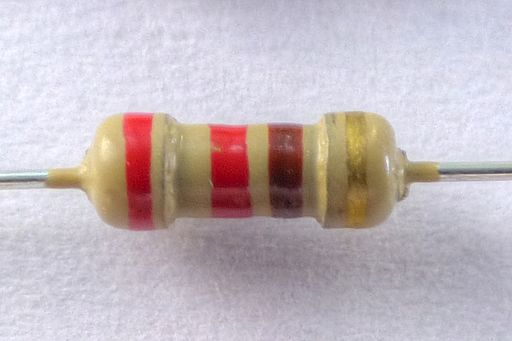
\includegraphics{./graphics-uncertainties/resistor.jpg}
  \caption{A resistor. \\ 
  \href{https://commons.wikimedia.org/wiki/File\%3AResistor_1480417_8_9_HDR_Enhancer_1.jpg}{220 Ohm resistor} by \href{https://commons.wikimedia.org/wiki/User:Nevit}{Nevit Dilmen} is licensed under \href{https://creativecommons.org/licenses/by-sa/3.0/deed.en}{CC BY-SA 3.0}.}
  \label{fig:resistor}
\end{marginfigure}

In the case of a measuring instrument, the manufacturer's data sheet
may also provide an estimate of the relative uncertainty for measurements made
with that instrument. 

The other way to estimate the measurement uncertainty is using the
smallest interval that the instrument measures. For instance, a ruler
may have marks spaced by a millimeter. In that case, we give the
measurement to the nearest millimeter (e.g. 93 mm), and the
uncertainty as $0.5$ mm. In general, for an analog instrument the rule
would be to use half the smallest division. 

If we are using a digital instrument, the uncertainty is half the last
significant digit. Thus, if your voltmeter is showing 9.75 Volts, the
uncertainty is estimated to be 0.005 Volts. 

\section{Uncertainty propagation}
Very often, we measure a quantity to calculate something. For example,
the volume of a cylinder of diameter $D$ and length $L$ is 
\begin{equation}
  \label{eq:errors_2}
  V=\pi\frac{D^2}{4}L
\end{equation}
We measure the diameter and the length with their uncertainties,
$u(D)$ and $u(L)$; what is the resulting uncertainty in the volume
$u(V)$?

According to GUM, if we have a function $y(x_1,x_2,\cdots,x_N)$ where
the $x_i$ are measured with uncertainties $u(x_i)$, the uncertainty in
the calculated value $y$ is given by
\begin{equation}
  \label{eq:errors_3}
  u(y)=\sqrt{c_1^2u(x_1)^2+c_2^2u(x_2)^2+\cdots c_N^2u(x_N)^2}
\end{equation}
where the $c_i$ are called \textbf{sensitivity coefficients}, because
they express how sensitive $y$ is to uncertainties in each of the
variables. 

The sensitivity coefficients are just the \textbf{partial derivatives}
of $y$ with respect to each $x_i$:
\begin{equation}
  \label{eq:errors_4}
  c_i=\frac{\partial y}{\partial x_i}
\end{equation}

For an explanation of the concept of partial derivative, please see
 appendix \ref{app:partial} before continuing.

You can see why the $c_i$ are called sensitivity coefficients. Since
they are multiplying the respective uncertainties, they determine how
sensitive the measurement of $y$ is to uncertainties in the
measurement of each variable. If a sensitivity coefficient is very
high compared with the others, that tells us that the corresponding
variable weighs very heavily in overall uncertainty. In that case, we
may want to measure that particular variable with a more precise
instrument, to reduce its uncertainty. 

In our example of the cylinder, $V$ is a function of $D$ and $L$, with
\begin{eqnarray}
  \label{eq:errors_5}
  \frac{\partial V}{\partial D}&=&\frac{\pi}{2}DL\\
  \frac{\partial V}{\partial L}&=&\pi\frac{D^2}{4}
\end{eqnarray}
Then the uncertainty in $V$ is given by
\begin{equation}
  \label{eq:errors_6}
  u(V)=\sqrt{\left(\frac{\pi}{2}DL\right)^2u(D)^2+\left(\pi\frac{D^2}{4}\right)^2u(L)^2}
\end{equation}

\section{Sums and products}

The uncertainty propagation formula takes on a particularly simple
form when the function is a sum or a product of several variables.

If
\begin{equation}
  \label{eq:errors_7}
  y=A_1x_1+A_2x_2+\cdots +A_Nx_N
\end{equation}
then each $c_i=A_i$, and 
\begin{equation}
  \label{eq:errors_8}
  u(y)=\sqrt{A_1^2u(x_1)^2+A_2^2u(x_2)^2+\cdots +A_N^2u(x_N)^2}
\end{equation}

For example, the perimeter of a rectangle of sides $a$ and $b$ is
$P=2a+2b$. The uncertainty in the perimeter $u(P)$ is
\begin{equation}
  \label{eq:errors_8_1}
  u(P)=\sqrt{4u(a)^2+4u(b)^2}
\end{equation}

More interesting perhaps is the case where
\begin{equation}
  \label{eq:errors_9}
  y=Ax_1^{n_1}x_2^{n_2}\cdots x_N^{n_N}
\end{equation}
Here the sensitivity coefficients are given by
\begin{equation}
  \label{eq:errors_10}
  \frac{\partial y}{\partial x_i}=n_i\frac{y}{x_i}
\end{equation}
so that
\begin{equation}
  \label{eq:errors_11}
  u(y)=\sqrt{n_1^2\left(\frac{y}{x_1}\right)^2u(x_1)^2+n_2^2\left(\frac{y}{x_2}\right)^2u(x_2)^2+\cdots
  n_N^2\left(\frac{y}{x_N}\right)^2u(x_N)^2}
\end{equation}
Now divide by $y$, and remember that $u(y)/y$ is the relative
uncertainty $w(y)$, and in the same way $u(x_i)/x_i$ is the relative
uncertainty $w(x_i)$:
\begin{equation}
  \label{eq:errors_12}
  w(y)=\sqrt{n_1^2w(x_1)^2+n_2^2w(x_2)^2+\cdots +n_N^2w(x_N)^2}
\end{equation}

So in the case of a product, it is most convenient to deal with the
relative uncertainties. Recall the volume of the cylinder discussed
earlier:
\begin{equation}
  \label{eq:errors_13}
    V=\pi\frac{D^2}{4}L
\end{equation}
Applying equation (\ref{eq:errors_12}), we find the relative
uncertainty in the volume to be
\begin{equation}
  \label{eq:errors_14}
  w(V)=\sqrt{4w(D)^2+w(L)^2}
\end{equation}
Notice how simple and yet informative this result is. It is clear that the
relative uncertainty in the diameter weighs significantly more (four
times more to be exact) than the relative uncertainty in the
length. Maybe we should measure the diameter with special care. 

Very often the expressions we have to deal with are products of powers
of variables. If that's the case, then we should look for the relative
uncertainty right away.

\section{An electrical example}
One more example. We are presented with a resistor and a voltage
source, and asked to measure the power dissipated by the resistor. The
value of the resistance and its relative uncertainty is encoded on the
resistor itself. The value of the voltage across
the resistor is measured with a voltmeter. Find the relative
uncertainty and the standard uncertainty of the power.

Here is a checklist of the procedure:
\begin{enumerate}
\item 
Write the calculated quantity as a function of the measured variables.
\begin{quote}
  \begin{equation}
    \label{eq:errors_15}
    P=\frac{V^2}{R}
  \end{equation}
\end{quote}
\item
Measure and estimate the uncertainty or the relative uncertainty of
each of the measured variables. Give the uncertainties to at most 2
significant figures. 
\begin{quote}
  The value of the resistance and its relative uncertainty is encoded
  on the resistor: $120\Omega\pm 5$\%. The voltage is measured with a
  voltmeter that provides 4 significant figures, so we take half the
  smallest significant figure as the uncertainty: $(6.750\pm 0.0005)$
  V. Since the power is a product of powers of $V$ and $R$, we will
  need the relative uncertainties. The relative uncertainty of the
  resistance is already given. For the voltage we calculate it as
  \begin{equation}
    \label{eq:errors_16}
    w(V)=\frac{u(V)}{V}=7.4\times 10^{-3}\%
  \end{equation}
\end{quote}
\item
  Write the error propagation formula for the quantities involved in
  the problem, and calculate the desired uncertainty.
  \begin{quote}
    \begin{equation}
      \label{eq:errors_17}
      w(P)=\sqrt{4w(V)^2+w(R)^2}=5\%
    \end{equation}

Notice that this is essentially the same as the relative uncertainty of the
resistance! The precision of the voltmeter is such that the
uncertainty of the voltage is negligible by comparison. If we wanted a
more precise result, we would concentrate our efforts on measuring the
resistance with a smaller uncertainty, rather than merely reading the
label. 
  \end{quote}
\item
  Calculate the desired quantity itself and report the result. Make
  sure that the value of the quantity is not given with more
  significant figures than is warranted by the experimental uncertainty.
  \begin{quote}
    If I enter the measured values of R and V in my calculator and
    calculate the power, it gives me a value of 0.3796875 Watts. But
    are all those digits really justified? The relative uncertainty is
    5\%, or about 0.02 Watts. So already the 9 in 0.379 is a lie! We
    report the final result as
    \begin{equation}
      \label{eq:errors_18}
      P=0.38~\mbox{W}\pm 5\% 
    \end{equation}
    or
    \begin{equation}
      \label{eq:errors_19}
      P=(0.38\pm 0.02)~\mbox{W}
    \end{equation}
  \end{quote}
\end{enumerate}
\clearpage

\begin{appendices}
\section{Partial derivatives}\label{app:partial}
The partial derivative, as you can imagine, is an extension of the
concept of derivative to functions of more than one variable. Think of
such a function as $y=f(x_1,x_2,\ldots x_N)$. The partial derivative
with respect to $x_i$
is the answer to the question ``How does $y$ change when I change the
variable $x_i$ \textit{only}?''. It is calculated by pretending that
all the other variables in the expression for $y$ are constant,
reducing the problem to one variable only. The notation for the
partial derivative with respect to $x_i$ is
\begin{equation}
  \label{eq:errors_20}
  \frac{\partial f}{\partial x_i}
\end{equation}
For example, say $y=3x_1^4/x_2$. The partial derivatives of $y$ with
respect to $x_1$ and $x_2$ are
\begin{eqnarray}
  \label{eq:errors_21}
  \frac{\partial f}{\partial x_1}&=&\frac{12x_1^3}{x_2}\\
  \frac{\partial f}{\partial x_2}&=&-\frac{3x_1^4}{x_2^2}
\end{eqnarray}
\end{appendices}
\clearpage

\section*{Exercises}
\begin{enumerate}
\item
The volume of a sphere is 
\begin{equation*}
V=\frac{4}{3}\pi R^3
\end{equation*}
If the measured radius of a sphere is $R=3.0$ cm, with a relative uncertainty $w(R)=2$\%, calculate its volume $V$, with its relative uncertainty $w(V)$.

\item
\begin{enumerate}
\item
Alice measures the length of a sheet of paper with a ruler whose smallest division is 1 mm. The measured length is $L=27.9$ cm. What is the standard uncertainty in the length, $u(L)$? What is the relative uncertainty in the length, $w(L)$?
\item
Alice then measures the width of the sheet of paper with the same ruler, and finds $W=21.6$ cm. With these data, she calculates the area of the sheet of paper, $A=LW$. What is the calculated value of $A$? What are the values of the sensitivity coefficients $\partial A/\partial L$ and $\partial A/\partial W$? Finally, using the error propagation formula, what is the standard uncertainty in the area, $u(A)$? What is the relative uncertainty in the area, $w(A)$?
\end{enumerate}


\item
\begin{enumerate}
\item
Bob measures the focal length $f$ of a converging lens by placing an object at a distance $s$ from the lens, and measuring the distance $s'$ to a screen on the other side of the lens, where a sharp image is formed. According to the thin lens equation, 
\begin{equation*}
\frac{1}{s}+\frac{1}{s'}=\frac{1}{f}
\end{equation*}

For an object distance $s=(40.0\pm 0.1)$ cm, Bob finds $s'=(13.5\pm 0.1)$ cm. Calculate the focal length $f$ and its standard uncertainty. 
\item
Bob finds the spec sheet for the lens, where it says that the focal length is 10 cm. Does this agree with his measured value of $f$, within the experimental uncertainty?
\end{enumerate}
\end{enumerate}
\end{document}